\documentclass[sigconf]{acmart}

\settopmatter{printacmref=true}
\renewcommand\footnotetextcopyrightpermission[1]{}

\setcopyright{none}

\acmConference[SBES 2026]{40th Brazilian Symposium on Software Engineering}{September 8–11, 2026}{São Paulo, SP, Brazil}

\AtBeginDocument{
    \providecommand\BibTeX{{Bib\TeX}}
}

% Reconfigurações para artigos em PORTUGUÊS
\renewcommand\abstractname{Resumo}
\renewcommand\keywordsname{Palavras-chave}
\renewcommand\refname{Referências}

\begin{document}

\title{Níveis de Instrumentação e seu Impacto na Observabilidade: Uma Revisão da Literatura Científica}

\author{Fagner Silva}
\affiliation{
  \institution{Centro de Informática, UFPE}
  \city{Recife}
  \country{Brasil}
}
\email{ffcs@cin.ufpe.br}

\author{Jackson Raniel}
\affiliation{
  \institution{Universidade de Pernambuco - Campus Caruaru}
  \city{Caruaru}
  \country{Brasil}
}
\email{jackson.florencio@upe.br}

\author{Vinícius Cardoso Garcia}
\affiliation{
  \institution{Centro de Informática, UFPE}
  \city{Recife}
  \country{Brasil}
}
\email{vcg@cin.ufpe.br}

\renewcommand{\shortauthors}{Silva et al.}
\renewcommand{\shorttitle}{Níveis de Instrumentação e seu Impacto na Observabilidade}

\frenchspacing

\begin{abstract}
Sistemas distribuídos modernos, aplicações nativas da nuvem e ambientes de computação de alto desempenho exigem observabilidade abrangente para garantir a confiabilidade, diagnosticar anomalias de desempenho e otimizar a utilização de recursos. A observabilidade depende fundamentalmente da instrumentação em múltiplas camadas do sistema, onde cada camada introduz compromissos (\textit{trade-offs}) críticos entre profundidade de visibilidade, sobrecarga de desempenho e capacidade diagnóstica. Esta revisão de literatura examina sistematicamente o panorama dos níveis de instrumentação e seus efeitos na observabilidade e no uso de recursos. Analisamos 19 artigos revisados por pares para responder a três questões de pesquisa: mapeamento dos níveis de instrumentação, quantificação do impacto no desempenho e identificação de melhores práticas para minimizar a sobrecarga. Nossos achados revelam uma transição paradigmática de perfis estáticos para abordagens dinâmicas, adaptativas e conscientes de custos. Estruturas dinâmicas como o DTrace atingem sobrecarga próxima de zero quando desativadas, soluções em hardware eliminam artefatos de software na análise de ameaças e estratégias multinível direcionam dinamicamente os recursos de monitoramento durante anomalias. Por fim, esta síntese fornece diretrizes de design e aponta direções futuras, como monitoramento adaptativo guiado por aprendizado de máquina e instrumentação consciente do consumo energético.
\end{abstract}

\keywords{Observabilidade, Níveis de Instrumentação, Sobrecarga de Desempenho, Revisão Rápida}

\maketitle

\section{Introdução}

Sistemas distribuídos modernos, aplicações nativas da nuvem e ambientes de computação de alto desempenho exigem observabilidade abrangente para garantir a confiabilidade, diagnosticar problemas de desempenho e otimizar a utilização de recursos. A observabilidade — a capacidade de inferir os estados internos de um sistema a partir de suas saídas e emissões de telemetria externas — depende fundamentalmente da instrumentação: a inserção de pontos de medição e sondas (\textit{probes}) que capturam dados de execução, consumo de recursos e padrões comportamentais. No entanto, a instrumentação não é um conceito monolítico; ela pode ser aplicada em múltiplas camadas da pilha computacional, cada uma com características distintas em relação à profundidade de visibilidade, sobrecarga de desempenho (\textit{overhead}) e capacidade diagnóstica.

A escolha do nível de instrumentação representa uma decisão arquitetural crítica com implicações de longo alcance. A instrumentação de grão fino em nível de aplicação pode expor informações semânticas detalhadas sobre a lógica de negócios e estados de variáveis, enquanto o rastreamento em nível de kernel revela a utilização de recursos em todo o sistema operacional e o comportamento do escalonamento de processos. Abordagens baseadas em hardware podem eliminar completamente os artefatos de software, e \textit{frameworks} adaptativos ajustam dinamicamente a intensidade do monitoramento com base nas condições operacionais do sistema. Cada abordagem impõe compromissos (\textit{trade-offs}) inerentes entre a profundidade da observabilidade e a perturbação induzida no desempenho.

Embora levantamentos recentes na literatura abordem aspectos pontuais da telemetria moderna — concentrando-se predominantemente no rastreamento distribuído exclusivo para microsserviços em nuvem ou na aplicação especializada do eBPF em sistemas operacionais —, nota-se uma carência de estudos secundários que tracem um panorama comparativo e vertical abrangente. Persiste uma lacuna de investigações que cruzem sistematicamente as diferentes camadas de abstração do sistema (desde o silício até o código de aplicação), confrontando a riqueza diagnóstica obtida com a quantificação empírica de seus impactos computacionais (latência, utilização de CPU, memória e consumo energético).

Para preencher essa lacuna, esta revisão de literatura examina sistematicamente o panorama dos níveis de instrumentação e seus efeitos na observabilidade e no desempenho do sistema. Analisamos 19 artigos primários revisados por pares para responder a três questões centrais de pesquisa:
\begin{itemize}
    \item \textbf{RQ01:} Quais níveis de instrumentação existem e quais características de observabilidade cada um fornece?
    \item \textbf{RQ02:} Como diferentes abordagens de instrumentação impactam o desempenho do sistema e a utilização de recursos?
    \item \textbf{RQ03:} Quais estratégias e melhores práticas permitem uma observabilidade eficaz minimizando a sobrecarga de desempenho?
\end{itemize}

Ao sintetizar evidências empíricas e modelos conceituais reportados na literatura recente, esta revisão fornece um arcabouço estruturado para orientar engenheiros e pesquisadores na seleção consciente de técnicas de monitoramento. O restante deste artigo está estruturado da seguinte forma: a Seção~\ref{sec:fund-teorica} discute a fundamentação teórica; a Seção~3 apresenta a metodologia e o protocolo da revisão rápida; a Seção~\ref{sec:niveis-instrumentacao} detalha a taxonomia dos níveis de instrumentação identificados (RQ01); a Seção~\ref{sec:observabilidade-impacto} analisa os impactos na observabilidade, overhead e técnicas adaptativas (RQ02 e RQ03); a Seção~6 sintetiza as discussões e direções de pesquisas futuras; e a Seção~7 conclui o trabalho.

\section{Fundamentação Teórica}
\label{sec:fund-teorica}

A instrumentação computacional constitui o alicerce para a medição de desempenho, depuração e compreensão do comportamento dinâmico de sistemas \cite{waheed_instrumentation}. Contudo, a inserção de código de monitoramento é historicamente limitada pelo chamado ``efeito de sonda'' (\textit{probe effect}) ou princípio da incerteza da medição de software \cite{sivasubramaniam_1994, garcia_2000}. Esse fenômeno estabelece que o ato de observar um sistema inevitavelmente altera seu comportamento temporal e espacial: a execução das sondas consome ciclos de processamento, polui as linhas de memória cache, introduz contenção em primitivas de sincronização e pode mascarar ou induzir anomalias artificiais (como condições de corrida e variações de latência) que não ocorreriam na execução não monitorada \cite{sivasubramaniam_1994}.

A gravidade do efeito de sonda está intimamente associada à chamada ``lacuna semântica'' (\textit{semantic gap}), formalizada no trabalho pioneiro de Shende et al. \cite{shende_2001}. Os autores observaram que as camadas sucessivas de abstração — tais como hardware, sistemas operacionais, máquinas virtuais e interpretadores — criam uma distância conceitual entre a execução física das instruções e a lógica de negócios da aplicação. Essa lacuna impõe um dilema fundamental no projeto de observabilidade: camadas inferiores (hardware e kernel) fornecem medições microscópicas e com mínima perturbação temporal, mas são semanticamente cegas em relação ao fluxo transacional da aplicação; por outro lado, camadas superiores (código-fonte e bytecode) capturam a semântica completa das operações ao custo de maior intrusão e expressivo \textit{overhead} computacional \cite{shende_2001, debes_application}.

A evolução histórica da instrumentação reflete os esforços da Engenharia de Software para mitigar essa lacuna semântica sem inviabilizar o desempenho em produção. As abordagens tradicionais das décadas de 1970 a 1990 focavam em instrumentação estática em tempo de compilação para sistemas procedurais e paralelos homogêneos \cite{sivasubramaniam_1994}. No entanto, a consolidação de arquiteturas distribuídas, computação em nuvem e microsserviços introduziu novos desafios que tornaram a instrumentação estática proibitiva: a impossibilidade de paradas programadas (\textit{zero downtime}), a heterogeneidade das pilhas tecnológicas e a volatilidade das cargas de trabalho. Esses fatores impulsionaram o desenvolvimento de mecanismos de instrumentação dinâmica e interceptação baseada em \textit{middleware} \cite{reilly_2006}, permitindo a injeção e remoção de sondas sob demanda sem recompilação ou interrupção dos serviços.

Com base nesse corpo teórico, os compromissos de observabilidade podem ser estruturados em quatro dimensões fundamentais, governadas pelo \textbf{Princípio da Ortogonalidade} aplicado à taxonomia e ao projeto de sistemas computacionais \cite{nickerson_2013}. Em Engenharia de Software e arquitetura de sistemas, a ortogonalidade postula que as dimensões de um modelo devem ser conceituadas de modo independente e não redundante, garantindo que uma escolha arquitetural em um determinado eixo possa ser realizada sem impor restrições ou acoplamentos espúrios sobre os demais eixos. Nesse sentido, a estruturação multidimensional da observabilidade desdobra-se em quatro eixos ortogonais:
\begin{enumerate}
    \item \textbf{Camada do Sistema (Eixo Espacial):} a posição na pilha arquitetural onde as medições ocorrem (hardware, kernel, runtime de linguagem ou código de aplicação);
    \item \textbf{Características Temporais (Eixo de Vinculação):} o momento de inserção e ativação das sondas, variando de vinculação estática em tempo de compilação a instrumentação dinâmica em tempo de execução sem reinicialização;
    \item \textbf{Granularidade dos Dados (Eixo de Resolução):} a densidade da telemetria produzida, oscilando de contadores agregados de baixo custo (\textit{coarse-grained}) até rastreamentos evento a evento com retenção de contexto de chamada (\textit{fine-grained});
    \item \textbf{Política de Ativação (Eixo Operacional):} o regime de funcionamento das medições, alternando entre monitoramento ininterrupto (\textit{always-on}) e amostragem adaptativa ou sob demanda orientada por desvios de desempenho (\textit{cost-aware}).
\end{enumerate}
A adoção explícita do Princípio da Ortogonalidade \cite{nickerson_2013} assegura que o espaço de soluções de observabilidade seja formulado como um produto cartesiano desses eixos. Isso esclarece por que avanços tecnológicos recentes — como o eBPF no kernel ou os agentes dinâmicos de bytecode — combinam pontos distintos dessas dimensões (e.g., sondas dinâmicas de grão fino no kernel ativadas sob demanda), desacoplando a localização física da sonda de sua política de amostragem.

\section{Metodologia}

As Revisões Rápidas (\textit{Rapid Reviews} - RRs) são estudos secundários projetados para fornecer evidências científicas de forma tempestiva, apoiando a tomada de decisão em ambientes práticos e dinâmicos. Diferente das Revisões Sistemáticas da Literatura (RSL) tradicionais, as RRs otimizam o processo de busca e extração de dados considerando restrições de tempo e esforço, sem comprometer o rigor metodológico. 

Esta abordagem é particularmente adequada para este estudo, pois permite sintetizar rapidamente as evidências emergentes sobre os níveis de instrumentação e seus impactos na observabilidade e no desempenho computacional, preenchendo uma lacuna essencial entre a pesquisa acadêmica e a engenharia de sistemas aplicada. O processo desta RR foi conduzido em três fases principais: planejamento, execução e extração, detalhadas nas subseções a seguir.

\subsection{Fase de Planejamento}

Durante a fase de planejamento, foi estabelecido um protocolo estruturado baseado nas diretrizes de Cartaxo et al. \cite{cartaxo_2018}. Este protocolo definiu o problema de pesquisa, a estratégia de busca, os critérios de seleção e o procedimento de extração de dados. Para garantir a transparência e a reprodutibilidade, a ferramenta online \textit{Parsifal} foi utilizada para gerenciar todas as etapas do protocolo.

O objetivo deste estudo é mapear o panorama atual das abordagens de instrumentação, analisando suas capacidades diagnósticas e os compromissos (\textit{trade-offs}) em relação ao consumo de recursos. Para guiar a revisão, foram formuladas as seguintes Questões de Pesquisa (RQs):

\begin{itemize}
    \item \textbf{RQ01:} Quais níveis de instrumentação existem e quais características de observabilidade cada um fornece?
    \item \textbf{RQ02:} Como diferentes abordagens de instrumentação impactam o desempenho do sistema e a utilização de recursos?
    \item \textbf{RQ03:} Quais estratégias e melhores práticas permitem uma observabilidade eficaz minimizando a sobrecarga de desempenho?
\end{itemize}

\subsection{Fase de Execução}

A execução envolveu a busca sistemática na literatura utilizando quatro bases de dados científicas de relevância primária na área de Ciência da Computação e Engenharia de Software: IEEE Xplore, ACM Digital Library, SpringerLink e ScienceDirect. O recorte temporal foi estabelecido entre \textbf{2003} e \textbf{2025} para capturar as abordagens mais contemporâneas.

A \textit{string} de busca foi construída a partir dos conceitos centrais das RQs e adaptada para a sintaxe específica de cada base, aplicando o filtro de texto completo (\textit{full-text}):

\begin{quote}
\textbf{String de Busca:} \texttt{("observability" OR "monitoring") AND ("instrumentation" OR "profiling" OR "tracing") AND ("performance impact" OR "overhead" OR "resource utilization")}
\end{quote}

O fluxo de seleção e filtragem dos estudos seguiu as diretrizes do protocolo PRISMA (\textit{Preferred Reporting Items for Systematic Reviews and Meta-Analyses}), conforme ilustrado na Figura~\ref{fig:prisma_flow}. 

A busca inicial nas quatro bases de dados retornou um total de $N = 348$ artigos (IEEE Xplore: 124, ACM Digital Library: 102, SpringerLink: 76, ScienceDirect: 46). Na etapa de pré-processamento, foram identificados e removidos $N = 62$ estudos duplicados entre as bases, resultando em $N = 286$ artigos únicos para triagem.

\begin{figure*}[htbp]
\centering
\begin{tabular}{|c|}
\hline
\textbf{1. Identificação de Registros Nas Bases de Dados ($N = 348$)} \\
\small (IEEE Xplore: 124 | ACM Digital Library: 102 | SpringerLink: 76 | ScienceDirect: 46) \\
\hline
$\downarrow$ \\
\hline
\textbf{2. Remoção de Estudos Duplicados ($N = 62$ Excluídos $\rightarrow$ $N = 286$ Restantes)} \\
\hline
$\downarrow$ \\
\hline
\textbf{3. Triagem Inicial por Título e Resumo ($N = 286$ Avaliados)} \\
\small $\rightarrow$ $N = 224$ Excluídos (Fora do escopo principal ou sem avaliação de instrumentação) \\
\hline
$\downarrow$ \\
\hline
\textbf{4. Leitura do Texto Completo ($N = 62$ Avaliados na Íntegra)} \\
\small $\rightarrow$ $N = 48$ Excluídos com justificativas: \\
\small • EC02 / EC04 (Artigos curtos/literatura cinzenta): $n = 18$ \\
\small • EC03 (Instrumentação apenas como ferramenta periférica): $n = 21$ \\
\small • Ausência de dados de overhead/desempenho: $n = 9$ \\
\hline
$\downarrow$ \\
\hline
\textbf{5. Adição via \textit{Snowballing} e Grafos de Citação (\textit{Research Rabbit}) ($N = +5$ Novos Estudos)} \\
\hline
$\downarrow$ \\
\hline
\textbf{6. Total Final de Estudos Primários Incluídos na Revisão ($N = 19$)} \\
\hline
\end{tabular}
\caption{Fluxo do Processo de Seleção e Filtragem de Estudos (Adaptado do Protocolo PRISMA).}
\Description{Diagrama mostrando o fluxo do Processo de Seleção e Filtragem de Estudos (Adaptado do Protocolo PRISMA).}
\label{fig:prisma_flow}
\end{figure*}

O processo de filtragem seguiu três etapas rigorosas:
\begin{enumerate}
    \item \textbf{Triagem Inicial:} Avaliação de títulos e resumos por um único pesquisador frente aos critérios IC/EC, resultando na exclusão de $N = 224$ trabalhos irrelevantes.
    \item \textbf{Revisão de Texto Completo:} Os $N = 62$ estudos retidos foram lidos na íntegra. Desses, $N = 48$ foram excluídos por motivos específicos: trabalhos curtos ou literatura cinzenta ($n = 18$), instrumentação tratada apenas como recurso secundário sem análise direta de suas propriedades ($n = 21$) e ausência de dados empíricos de \textit{overhead} ou recursos ($n = 9$).
    \item \textbf{Recuperação Adicional e Resolução de Conflitos:} Para expandir a cobertura e mitigar limitações da \textit{string} principal, aplicou-se \textit{Snowballing} (\textit{forward} e \textit{backward}) e busca gráfica pelo \textit{Research Rabbit}, adicionando $N = 5$ estudos elegíveis. Em casos de incerteza quanto à inclusão, um segundo pesquisador foi consultado para a decisão final de consenso, resultando no corpus final de $N = 19$ artigos primários.
\end{enumerate}

\subsection{Fase de Extração e Relatório}

Para cada estudo selecionado na etapa anterior, os dados foram extraídos sistematicamente por um pesquisador e validados de forma cruzada por um segundo autor utilizando os formulários estruturados do \textit{Parsifal}. O mapeamento dos dados extraídos seguiu o alinhamento direto com as Questões de Pesquisa: definições e capacidades operacionais das camadas (para a \textbf{RQ01}); quantificações de latência, CPU e memória (para a \textbf{RQ02}); e propostas de arquiteturas adaptativas ou \textit{frameworks} conscientes de custos (para a \textbf{RQ03}). A fase de relatório consistiu na síntese qualitativa e comparativa dessas informações para compor as discussões estabelecidas nas seções seguintes.

\subsection{Ameaças à Validade}
\label{sec:ameacas-validade}

A condução desta Revisão Rápida envolveu escolhas metodológicas orientadas pelo equilíbrio entre a tempestividade da entrega e o rigor científico necessário para apoiar decisões práticas \cite{cartaxo_2018}. Para assegurar a credibilidade e a transparência dos achados, as potenciais ameaças à validade foram identificadas, estruturadas e tratadas com base no esquema taxonômico de Wohlin et al. \cite{wohlin_2012}:

\begin{itemize}
    \item \textbf{Validade de Construto:} Trata da adequação entre os conceitos teóricos investigados e as medidas operacionais aplicadas \cite{wohlin_2012}. O viés de delimitação do escopo da busca foi mitigado formulando uma \textit{string} com múltiplos sinônimos cobrindo observabilidade, monitoramento, \textit{tracing}, \textit{profiling} e impacto computacional. Além disso, a aplicação de \textit{Snowballing} e a descoberta baseada em grafos de citação (\textit{Research Rabbit}) permitiram capturar estudos relevantes que utilizavam terminologias alternativas.
    
    \item \textbf{Validade Interna:} Refere-se a fatores e vieses não controlados que podem ter afetado a seleção e a extração dos dados \cite{wohlin_2012}. A condução da triagem inicial por apenas um pesquisador representa uma limitação intrínseca ao formato de Revisão Rápida \cite{cartaxo_2018}. Para mitigar esse viés, a fase de avaliação do texto completo e a resolução de casos ambíguos contaram com a revisão pareada e validação cruzada por um segundo autor. O uso da ferramenta \textit{Parsifal} assegurou a rastreabilidade e auditabilidade do protocolo.
    
    \item \textbf{Validade de Conclusão:} Refere-se à capacidade de extrair conclusões corretas a partir dos dados coletados \cite{wohlin_2012}. A acentuada heterogeneidade nas métricas de \textit{overhead} reportadas pelos artigos primários (variando entre incremento de latência, uso de CPU e degradação de vazão) inviabilizou a realização de uma síntese quantitativa ou meta-análise. Essa ameaça foi contornada adotando-se uma síntese qualitativa e uma categorização taxonômica baseada nas camadas de instrumentação e no comportamento temporal.
    
    \item \textbf{Validade Externa:} Diz respeito à amplitude e capacidade de generalização dos resultados obtidos \cite{wohlin_2012}. A limitação ao recorte temporal (2003--2025) e a seleção de quatro bases acadêmicas indexadas garantem representatividade na literatura científica de Engenharia de Software, embora possam ter desconsiderado relatos práticos presentes na literatura cinzenta (\textit{gray literature}) ou documentações comerciais de ferramentas recentes.
\end{itemize}

\section{Níveis de Instrumentação}
\label{sec:niveis-instrumentacao}

A observabilidade em sistemas computacionais modernos é viabilizada pela inserção de pontos de medição em diferentes camadas da pilha de execução \cite{shende_2001, cantrill_2004}. Cada camada oferece uma perspectiva distinta sobre o comportamento do sistema, estabelecendo um compromisso (\textit{trade-off}) inerente entre a riqueza semântica dos dados capturados, a profundidade de visibilidade e a sobrecarga (\textit{overhead}) de desempenho induzida \cite{haghshenas_2023, vysocky_2019}. Enquanto a instrumentação de grão grosso em níveis mais baixos favorece a cobertura global com baixo impacto, a visibilidade fina em níveis superiores expõe detalhes da lógica de negócios ao custo de maior perturbação \cite{ghanta_2017}. 

Sob a ótica do método taxonômico de Nickerson et al. \cite{nickerson_2013}, os quatro níveis de abstração identificados na literatura analisada ($N=19$) constituem a \textbf{dimensão espacial primária} da observabilidade. Essa hierarquia organiza-se desde os recursos físicos de silício até a semântica da aplicação de usuário, conforme esquematizado na Figura~\ref{fig:niveis_hierarchy}. As demais características operacionais (como vinculação dinâmica e amostragem adaptativa) operam como eixos ortogonais que qualificam o comportamento de cada ferramenta dentro de sua respectiva camada.

\begin{figure*}[t]
\centering
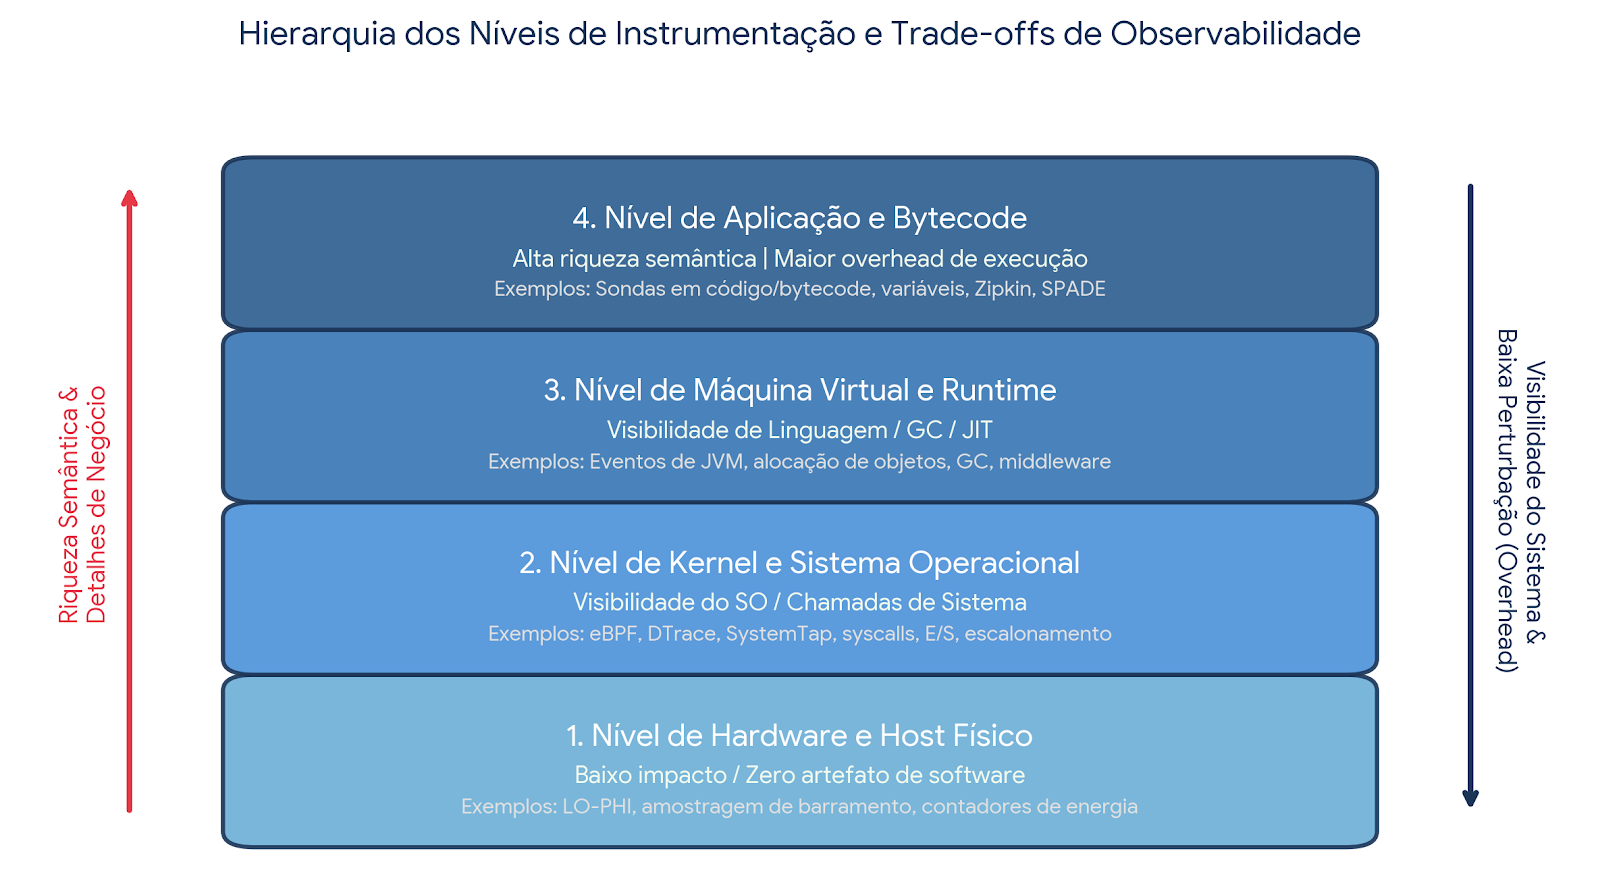
\includegraphics[width=\linewidth]{img/niveis_instrumentacao_hierarchy.png}
\caption{Hierarquia das camadas de instrumentação e seus compromissos (\textit{trade-offs}) entre riqueza semântica e sobrecarga computacional.}
\Description{Diagrama mostrando a hierarquia das camadas de instrumentação e os compromissos entre riqueza semântica e sobrecarga computacional.}
\label{fig:niveis_hierarchy}
\end{figure*}

\subsection{Instrumentação de Hardware e Host Físico}
A instrumentação de nível de hardware representa a camada mais baixa da hierarquia, operando abaixo da pilha de software para monitorar recursos físicos do sistema. Esta abordagem oferece vantagens únicas em termos de observação livre de artefatos e acesso abrangente ao estado.

O sistema LO-PHI (Low-Observable Physical Host Instrumentation) exemplifica a instrumentação baseada em hardware para análise de malware, fornecendo introspecção de máquina física tanto de memória não volátil (disco rígido) quanto volátil (memória do sistema) \cite{spensky_2016}. O LO-PHI expõe zero artefatos baseados em software e artefatos de hardware mínimos, mantendo capacidades de análise comparáveis às soluções baseadas em software existentes. Essa abordagem analisa significativamente mais binários do que as contrapartes de software porque não pode ser frustrada por técnicas populares de anti-análise. A medição de energia é outro domínio essencial; o trabalho de Ilsche em sistemas de computação de alto desempenho (HPC) quantificou a sobrecarga de medição de energia e o impacto nos recursos, fornecendo insights sobre a utilização de cargas de trabalho analisadas \cite{ilsche_2020}.

\subsection{Nível de Kernel e Sistema Operacional}
A instrumentação de nível de kernel fornece visibilidade sobre chamadas de sistema, decisões de escalonamento, operações de E/S e alocação de recursos.

O DTrace, introduzido por \cite{cantrill_2004} permite a instrumentação dinâmica de softwares de nível de usuário e kernel de forma unificada e segura. Quando não habilitado, o DTrace exibe "efeito de sondagem zero" — o sistema opera como se o DTrace não estivesse presente. O framework suporta dezenas de milhares de pontos de instrumentação, com sistemas pequenos oferecendo cerca de 30.000 pontos apenas no kernel. Tecnologias modernas como eBPF (extended Berkeley Packet Filter) continuam essa evolução. \cite{volpert_2025} quantifica as diferenças de sobrecarga entre eBPF e SystemTap, orientando a seleção de ferramentas para produção.

\subsection{Nível de Máquina Virtual e Runtime}
A instrumentação de nível de VM e runtime visa a camada de execução da linguagem, capturando eventos específicos como coleta de lixo (garbage collection) e compilação JIT.

A pesquisa de \cite{ghanta_2017} sobre arquiteturas de observabilidade em camadas para sistemas baseados em JVM descreve a progressão da instrumentação de nível de VM para telemetria em escala de produção. O trabalho analisa o impacto no tempo de resposta e no uso de CPU/memória, fornecendo evidências empíricas dos compromissos inerentes. A instrumentação de runtime permite rastrear padrões de alocação de objetos e eventos de sincronização de threads que são opacos ao nível do kernel.

\subsection{Nível de Aplicação e Bytecode}
Este nível insere pontos de medição diretamente no código-fonte ou no bytecode, oferecendo a maior riqueza semântica, mas geralmente com a maior sobrecarga.

\cite{vysocky_2019} discute que aplicações complexas mostram comportamentos diferentes em cada parte do código, tornando desejável a instrumentação para separar essas seções e identificar "pontos quentes" (hot spots) de consumo de recursos. \cite{wang_2025} descrevem a melhoria da observabilidade de serviços através do monitoramento de variáveis em nível de bytecode, suportando instrumentação estática e dinâmica. O sistema SPADE \cite{brown_2003} coleta dados de monitoramento de todos os níveis, incluindo a aplicação, e os armazena em um banco de dados relacional, permitindo correlacionar dados com solicitações semânticas da aplicação. \cite{yang_2025} estenderam a programabilidade e observabilidade do eBPF para GPUs, fornecendo múltiplas granularidades de instrumentação ligadas à profundidade de visibilidade e latência.

\section{Impacto na Observabilidade}
\label{sec:observabilidade-impacto}

Com relação ao impacto, a profundidade de visibilidade e cobertura sobre a observabilidade, a escolha do nível de instrumentação determina fundamentalmente quais aspectos do comportamento do sistema se tornam observáveis. Diferentes níveis expõem diferentes tipos de eventos, criando uma arquitetura de observabilidade em camadas onde cada camada contribui com insights únicos.

A instrumentação de kernel e de sistema operacional (SO) fornece visibilidade sobre a utilização de recursos em todo o sistema, decisões de escalonamento e padrões de E/S. A capacidade do DTrace de instrumentar tanto o código do kernel quanto o do nível de usuário de maneira unificada permite uma cobertura abrangente do comportamento do sistema \cite{cantrill_2004}. As dezenas de milhares de pontos de instrumentação do framework garantem que virtualmente qualquer evento de kernel ou de espaço de usuário possa ser observado quando necessário \cite{cantrill_2004}.

A instrumentação de aplicação e de bytecode expõe sinais semânticos e em nível de variável úteis para depuração e perfilamento (profiling) da lógica de negócios \cite{wang_2025}. A arquitetura de observabilidade em camadas de Ghanta \cite{ghanta_2017} demonstra como a instrumentação em nível de VM, de bytecode e de aplicação fornece uma visibilidade progressivamente mais refinada em sistemas baseados em JVM, com cada camada revelando diferentes aspectos do comportamento de execução.

A introspecção de hardware e de host pode revelar artefatos que a instrumentação puramente de software não detecta. A introspecção de máquina física do LO-PHI analisa com sucesso binários que frustram abordagens baseadas em software, demonstrando que a visibilidade em nível de hardware pode expor comportamentos deliberadamente ocultados de observadores em software \cite{spensky_2016}. Essa capacidade se mostra particularmente importante para análises de segurança e cenários de anti-evasão.

O sistema SPADE ilustra o poder da cobertura multinível \cite{brown_2003}. Ao coletar dados de monitoramento de todos os níveis do sistema, incluindo a aplicação, e correlacioná-los com requisições de aplicação semanticamente significativas, o SPADE permite a análise em múltiplos níveis de detalhe simultaneamente \cite{brown_2003}. Essa cobertura abrangente permite que os usuários localizem gargalos no sistema e testem hipóteses de desempenho sem a necessidade de múltiplas execuções de experimentos \cite{brown_2003}.

Com relação às capacidades diagnósticas, os diferentes níveis de instrumentação viabilizam diferentes classes de investigações diagnósticas. A capacidade diagnóstica de uma abordagem de instrumentação depende tanto dos tipos de eventos que ela pode observar quanto da riqueza semântica dos dados capturados.

A instrumentação em nível de kernel se destaca no diagnóstico de problemas de desempenho sistêmicos. Cantrill et al. relatam que o DTrace encontrou sérios problemas de desempenho sistêmico em sistemas de produção que não podiam ser encontrados usando recursos pré-existentes \cite{cantrill_2004}. Os mecanismos de agregação escaláveis e as capacidades de rastreamento especulativo do framework eliminam a necessidade da maior parte do pós-processamento, permitindo o diagnóstico em tempo real. O trabalho posterior de Cantrill descreve um caso em que um multiprocessador simétrico de 64 processadores exibiu misteriosos períodos de atividade do kernel que duravam minutos e faziam com que o desempenho dos benchmarks caísse drasticamente \cite{cantrill_2006}. Melhorias na observabilidade ao nível do kernel mostraram-se essenciais para diagnosticar tais problemas ocultos de desempenho.

A instrumentação em nível de aplicação permite o diagnóstico de problemas de lógica de negócios e problemas de desempenho específicos da aplicação. O rastreamento distribuído do Zipkin melhora significativamente a observabilidade do sistema em arquiteturas de microsserviços, permitindo que os desenvolvedores identifiquem gargalos de desempenho e resolvam problemas de forma mais eficiente \cite{marvis_2024}. A integração do rastreamento distribuído reduziu o tempo de depuração e aprimorou o monitoramento de desempenho entre os serviços.

A localização da causa raiz representa uma capacidade diagnóstica sofisticada. O sistema MicroRCA de Wu et al. localiza as causas raízes de problemas de desempenho em microsserviços correlacionando sintomas de desempenho da aplicação com a utilização de recursos do sistema, atingindo 89\% de precisão e 97\% de precisão média ponderada (\textit{mean average precision}) \cite{wu_2020}. Notavelmente, o MicroRCA realiza isso sem qualquer instrumentação da aplicação, baseando-se, em vez disso, em métricas de nível de sistema e em um modelo de grafo atribuído de propagação de anomalias.

A instrumentação adaptativa aprimora a capacidade diagnóstica ao direcionar-se dinamicamente a componentes problemáticos. O framework de Mos para monitoramento adaptativo usa modelos de execução para direcionar dinamicamente operações de perfilamento em componentes que exibem degradação de desempenho, garantindo um impacto negligenciável quando a aplicação-alvo funciona conforme o esperado e um impacto mínimo quando determinados componentes apresentam baixo desempenho \cite{mos_2004}.

\subsection{Granularidade e Agregação de Dados} 

A granularidade dos dados de instrumentação — desde resumos de grão grosso (\textit{coarse-grained}) até rastreamentos de eventos de grão fino (\textit{fine-grained}) — impacta significativamente tanto a eficácia da observabilidade quanto a sobrecarga (\textit{overhead}) do sistema. As estratégias de agregação determinam como os dados brutos de instrumentação são processados e apresentados.

\cite{haghshenas_2023} define camadas de instrumentação grossa e fina dentro de um framework consciente dos custos, quantificando seu efeito na profundidade de visibilidade e na latência. Cada camada está vinculada a impactos mensuráveis de desempenho e recursos, fornecendo uma abordagem sistemática para equilibrar os custos de instrumentação com insights de desempenho. Essa abordagem em camadas reconhece que diferentes cenários de diagnóstico exigem diferentes níveis de granularidade.

O mecanismo escalável do DTrace para agregação de dados aborda o desafio de gerenciar o alto volume de saída da instrumentação \cite{cantrill_2004}. Ao realizar a agregação na origem, em vez de exigir um pós-processamento extensivo, o DTrace reduz o \textit{overhead} associado à instrumentação de grão fino. Essa escolha de projeto permite que o framework suporte dezenas de milhares de pontos de instrumentação sem sobrecarregar o sistema com o volume de dados.

O framework \textit{Enhanced Cloud Observability} implementa tanto o log de grão grosso quanto o rastreamento de grão fino por meio de instrumentação dinâmica \cite{ramesh_2025}. Essa abordagem de dupla granularidade permite que os operadores usem logs leves para monitoramento contínuo, reservando o rastreamento detalhado de grão fino para investigações minuciosas de problemas específicos.

Brandt et al. demonstram que mesmo uma amostragem relativamente grossa pode fornecer insights valiosos. A abordagem de monitoramento de sistema desenvolvida por eles utilizando amostragem de 1Hz não teve impacto significativo nas aplicações, enquanto ainda conseguia resolver características de utilização de recursos \cite{brandt_2018}. Essa descoberta sugere que uma instrumentação de grão grosso cuidadosamente escolhida pode alcançar uma observabilidade aceitável com o mínimo de overhead.

O sistema EXIST de Wang et al. viabiliza uma observabilidade de rastreamento interna ao serviço extremamente eficiente em datacenters por meio de instrumentação de ultra-baixa sobrecarga \cite{wang_hou_2025}. Embora métricas específicas não tenham sido detalhadas nos metadados disponíveis, o trabalho demonstra que a instrumentação otimizada pode alcançar alta observabilidade com custos mínimos de desempenho.

A análise dos mecanismos de coleta de dados e de monitoramento revela que a busca por uma observabilidade abrangente está intrinsecamente atrelada à gestão de restrições de infraestrutura. Esta seção dedica-se a discutir as implicações práticas, os prós e os contras das abordagens mapeadas na literatura, estruturando-se em três eixos fundamentais. Primeiramente, examina-se a divergência operacional entre a instrumentação estática e a dinâmica, avaliando como o momento de inserção das sondas afeta a flexibilidade do sistema. Em seguida, analisa-se a quantificação do \textit{overhead}, consolidando o impacto empírico dessas ferramentas no consumo de recursos. Por fim, discutem-se as estratégias adaptativas e conscientes dos custos, que emergem como soluções sofisticadas para mitigar o impacto concorrencial entre monitoramento e desempenho computacional.

\subsection{Instrumentação Estática vs. Dinâmica}

As características temporais da instrumentação — se as sondas (probes) são inseridas permanentemente (estática) ou se podem ser ativadas e desativadas em tempo de execução (dinâmica) — afetam fundamentalmente o cálculo de compensação (trade-off) de desempenho.

A instrumentação estática impõe um perfil de overhead constante em sistemas de longa execução. Mos observa que a maioria das soluções de instrumentação exibe comportamento estático ao direcionar-se a um conjunto especificado de componentes e, para aplicações de longa execução, um perfil de sobrecarga constante é indesejável. Tipicamente, a instrumentação estática seria usada apenas durante uma auditoria de desempenho, sacrificando os benefícios de observar constantemente um sistema de produção em favor de um impacto reduzido no desempenho \cite{mos_2004}.

A instrumentação dinâmica aborda essa limitação permitindo a ativação e desativação de sondas em tempo de execução. O efeito zero de sonda do DTrace quando não ativado representa o caso ideal: o sistema opera exatamente como se a instrumentação não estivesse presente \cite{cantrill_2004}. Essa característica permite ao DTrace manter dezenas de milhares de pontos de instrumentação potenciais sem impor qualquer overhead até que sejam explicitamente ativados. A capacidade de adicionar com segurança muitos pontos de instrumentação sob demanda reduz o impacto em estado estacionário, preservando uma capacidade abrangente de observabilidade.

O framework de instrumentação dinâmica baseado em middleware de Reilly permite a inserção em tempo de execução de serviços de instrumentação sem tirar recursos do ar \cite{reilly_2006}. Essa capacidade se mostra essencial para aplicações distribuídas onde a instrumentação estática é impraticável devido à distribuição e à necessidade de flexibilidade em tempo de execução. Estudos de caso avaliando o framework avaliaram tanto a eficácia quanto o overhead de desempenho, demonstrando a viabilidade da instrumentação dinâmica em ambientes distribuídos.

A distinção entre instrumentação estática e dinâmica também se aplica ao nível de bytecode. O monitoramento de variáveis em nível de bytecode de Wang et al. suporta instrumentação tanto estática quanto dinâmica durante o uso, fornecendo flexibilidade na forma como a observabilidade é implantada e gerenciada \cite{wang_2025}.

\subsection{Quantificação de Sobrecarga/Overhead}

Quantificar o overhead da instrumentação é essencial para tomar decisões informadas entre observabilidade e desempenho. Diferentes abordagens e ferramentas de instrumentação exibem características de sobrecarga variadas.

Volpert et al. fornecem uma comparação exemplar do overhead do eBPF e do SystemTap, quantificando os custos de desempenho associados a esses frameworks de instrumentação dinâmica em nível de kernel \cite{volpert_2025}. Embora métricas específicas não tenham sido detalhadas nos metadados disponíveis, o trabalho demonstra que a escolha da ferramenta impacta significativamente a sobrecarga e que a medição empírica é necessária para guiar as decisões de implantação em produção.

O framework de monitoramento adaptativo de Mos demonstra um overhead negligenciável quando a aplicação-alvo funciona conforme o esperado, com impacto mínimo quando certos componentes apresentam baixo desempenho \cite{mos_2004}. Os resultados experimentais obtidos com o protótipo da ferramenta demonstram a viabilidade dessa abordagem em termos de sobrecarga induzida. Essa estratégia adaptativa transforma efetivamente o perfil de overhead de constante (como na instrumentação estática) para condicional (ativado apenas quando necessário).

Brandt et al. relatam que sua abordagem de monitoramento de sistema usando amostragem de 1Hz não teve impacto significativo nas aplicações \cite{brandt_2018}. Essa descoberta fornece um ponto de dados concreto: a amostragem a 1Hz — uma taxa suficiente para resolver características de utilização de recursos — impõe um overhead negligenciável.

O NEOS (Non-Intrusive Edge Observability Stack) de Kumar et al. reduz a quantidade de instrumentação de código necessária em até 80\% em comparação com a instrumentação manual \cite{kumar_2023}. Embora essa métrica aborde principalmente o esforço de desenvolvimento em vez do overhead em tempo de execução, a redução no código de instrumentação provavelmente se correlaciona com um menor impacto em tempo de execução.

A instrumentação baseada em hardware do LO-PHI fornece capacidades de análise comparáveis às soluções baseadas em software existentes, enquanto expõe zero artefatos baseados em software e mínimos artefatos de hardware \cite{spensky_2016}. Essa abordagem troca a complexidade de implementação por uma menor perturbação em tempo de execução, demonstrando que a instrumentação em nível de hardware pode minimizar o overhead visível pelo software.

\subsection{Abordagens Adaptativas e Conscientes dos Custos}

Estratégias de instrumentação adaptativas e conscientes dos custos representam abordagens sofisticadas para gerenciar a compensação entre observabilidade e desempenho. Essas técnicas ajustam dinamicamente a intensidade do monitoramento com base no comportamento do sistema ou modelam explicitamente o valor da informação contra o custo da instrumentação.

O framework consciente dos custos de Haghshenas et al. equilibra explicitamente os custos de instrumentação com os insights de desempenho \cite{haghshenas_2023}. O framework define camadas de instrumentação grossas e finas, quantificando seu efeito na profundidade de visibilidade e na latência, e vincula cada camada a impactos mensuráveis de desempenho e de recursos. Essa abordagem fornece uma metodologia sistemática para selecionar configurações de instrumentação que atendam aos objetivos de observabilidade dentro das restrições de recursos.

O framework de monitoramento adaptativo de Mos usa modelos de execução para direcionar dinamicamente as operações de perfilamento em componentes que exibem degradação de desempenho \cite{mos_2004}. Essa estratégia garante um overhead negligenciável durante a operação normal e aumenta a intensidade do monitoramento apenas quando necessário. A abordagem aborda o perfil de sobrecarga constante indesejável da instrumentação estática, tornando a intensidade do monitoramento responsiva ao comportamento do sistema.

O framework ENHANCED CLOUD OBSERVABILITY implementa instrumentação dinâmica com log de grão grosso e rastreamento de grão fino, conectando as escolhas de instrumentação à profundidade de visibilidade e aos impactos de desempenho \cite{ramesh_2025}. Essa abordagem multinível permite que os operadores mantenham um monitoramento contínuo leve, enquanto reservam a dispendiosa instrumentação de grão fino para investigações direcionadas.

Abordagens adaptativas reconhecem que nem todos os estados do sistema exigem o mesmo nível de observabilidade. Ao concentrar os recursos de instrumentação em componentes ou períodos de tempo problemáticos, essas estratégias alcançam melhores compensações gerais do que as abordagens de instrumentação uniforme. O principal desafio reside no desenvolvimento de heurísticas ou modelos eficazes para determinar quando e onde intensificar o monitoramento.

\section{Discussões e Trabalhos Futuros}

A Tabela~\ref{tab:analise_comparativa} sintetiza as principais características das abordagens de instrumentação analisadas na literatura ($N=19$), estruturando-as a partir da matriz taxonômica multidimensional. Fundamentada no Princípio da Ortogonalidade \cite{nickerson_2013}, a matriz de classificação desacopla a camada física de execução (nível do sistema) de suas propriedades temporais, estratégias de agregação e políticas adaptativas de custo. Essa abordagem permite aos projetistas identificar claramente os compromissos de cada proposta, comparando suas capacidades diagnósticas, a ordem de grandeza do impacto no desempenho e seus domínios primários de aplicação.

\begin{table*}[htbp]
\centering
\small
\setlength{\tabcolsep}{3pt}
\caption{Mapeamento Sintético e Comparativo das Abordagens de Instrumentação na Literatura ($N=19$)}
\label{tab:analise_comparativa}
\begin{tabular}{|p{0.13\textwidth}|p{0.15\textwidth}|p{0.25\textwidth}|p{0.17\textwidth}|p{0.14\textwidth}|p{0.09\textwidth}|}
\hline
\textbf{Nível / Camada} & \textbf{Ferramentas / Propostas} & \textbf{Características de Observabilidade} & \textbf{Impacto no Desempenho} & \textbf{Casos de Uso Principais} & \textbf{Ref. e Anos} \\ \hline

\textbf{Hardware \& Host Físico} & LO-PHI, Medição em HPC & Introspecção de memória volátil e não-volátil; zero artefatos de software; métricas de energia em nível de barramento. & Zero perturbação no software alvo; artefatos mínimos em hardware. & Análise de \textit{malware}, segurança cibernética e auditoria energética em HPC. & \cite{spensky_2016} (2016)\newline \cite{ilsche_2020} (2020) \\ \hline

\textbf{Kernel \& Sistema Operacional} & DTrace, eBPF, SystemTap, BPF Tools & Instrumentação unificada kernel/espaço de usuário; dezenas de milhares de sondas dinâmicas; rastreamento de syscalls e I/O. & Efeito de sonda zero quando inativo (DTrace); baixo \textit{overhead} e agregação na origem. & Diagnóstico sistêmico em produção; análise de latência e contenção de recursos. & \cite{cantrill_2004} (2004)\newline \cite{cantrill_2006} (2006)\newline \cite{gregg_2019} (2019)\newline \cite{volpert_2025} (2025) \\ \hline

\textbf{VM \& Runtime} & Arquiteturas JVM, Middleware Dinâmico & Rastreamento de alocação de objetos, compilação JIT, eventos de GC e sincronização de \textit{threads}. & \textit{Overhead} variável por camada; exige amostragem ou ativação condicional. & Telemetria em escala de produção; diagnóstico em sistemas Java/componentizados. & \cite{reilly_2006} (2006)\newline \cite{ghanta_2017} (2017) \\ \hline

\textbf{Aplicação \& Bytecode} & SPADE, Zipkin, eGPU, Bytecode Variable Monitoring, App Tuning & Visibilidade em nível de variável, rastreamento distribuído fim-a-fim de requisições, telemetria em GPUs e hot-spots de código. & \textit{Overhead} de médio a elevado; exige balanceamento rigoroso de granularidade. & Localização de causa raiz, microsserviços, depuração semântica e GPU \textit{offloading}. & \cite{brown_2003} (2003)\newline \cite{vysocky_2019} (2020)\newline \cite{marvis_2024} (2024)\newline \cite{wang_2025} (2025)\newline \cite{yang_2025} (2025) \\ \hline

\textbf{Adaptativo \& Consciente de Custos} & Cost-Aware Framework, Adaptive Monitoring, MicroRCA, NEOS, EXIST & Ativação sob demanda; amostragem adaptativa baseada em anomalias; correlação de métricas de SO sem alteração de código. & \textit{Overhead} negligenciável em operação normal; custo condicional durante falhas. & Ambientes de borda (\textit{Edge}), \textit{datacenters} e localização automatizada de causa raiz. & \cite{mos_2004} (2004)\newline \cite{wu_2020} (2020)\newline \cite{haghshenas_2023} (2023)\newline \cite{kumar_2023} (2023)\newline \cite{wang_hou_2025} (2025) \\ \hline

\textbf{Resiliência \& AIOps} & Cloud Resilience Architecture & Previsão de falhas com suporte a aprendizado de máquina e mitigação proativa de anomalias. & Custos computacionais deslocados para algoritmos preditivos fora do caminho crítico. & Sistemas de alta disponibilidade na nuvem e resiliência preditiva. & \cite{jalukuri_2025} (2025) \\ \hline
\end{tabular}
\end{table*}

Com base na literatura sintetizada, surgem várias melhores práticas para o projeto e a implantação de sistemas de instrumentação que equilibram a observabilidade com o desempenho.

Adequar o nível de instrumentação à necessidade diagnóstica: Instrumente a camada mais grossa (coarse) que ainda forneça o sinal necessário para minimizar o volume de dados e a intervenção \cite{vysocky_2019}. Para problemas de desempenho sistêmicos, a instrumentação em nível de kernel pode ser suficiente \cite{cantrill_2004}, enquanto problemas específicos da aplicação podem exigir visibilidade em nível de bytecode ou de aplicação \cite{wang_2025, marvis_2024}.

Preferir a instrumentação dinâmica à estática: A instrumentação dinâmica permite uma operação com overhead zero quando não está em uso, preservando uma capacidade abrangente de observabilidade \cite{cantrill_2004}. Essa abordagem permite que os sistemas mantenham extensos pontos de instrumentação sem impor uma sobrecarga constante \cite{cantrill_2004}.

Empregar estratégias de ativação adaptativa: Ative as sondas (probes) apenas ao investigar anomalias ou direcione a amostragem para componentes problemáticos para evitar o overhead constante \cite{mos_2004, haghshenas_2023}. O monitoramento adaptativo que ativa o perfilamento apenas para componentes com mau funcionamento pode manter a sobrecarga negligenciável durante a operação normal \cite{mos_2004}.

Aproveitar a agregação e o pré-processamento: Utilize a agregação no kernel (in-kernel) ou no processo (in-process) para reduzir a telemetria exportada e os custos de pós-processamento \cite{cantrill_2004}. O mecanismo de agregação escalável do DTrace demonstra como o processamento na origem pode gerenciar dados de instrumentação de alto volume \cite{cantrill_2004}.

Considerar arquiteturas de instrumentação multinível: Combine a instrumentação em múltiplos níveis para alcançar uma observabilidade abrangente \cite{ghanta_2017, brown_2003}. A abordagem multinível do SPADE com correspondência automática de granularidade mostra como diferentes camadas podem ser integradas de forma eficaz \cite{brown_2003}.

Aplicar a seleção consciente dos custos: Adote políticas de instrumentação conscientes dos custos que troquem a fidelidade do sinal pelo orçamento de recursos e priorizem as medições de maior valor sob restrições de recursos \cite{haghshenas_2023}. Modelar explicitamente a compensação (trade-off) custo-benefício permite uma otimização sistemática \cite{haghshenas_2023}.

Usar instrumentação de hardware para observação livre de artefatos: Quando os artefatos de software forem problemáticos (e.g., análise de segurança, cenários de anti-evasão), a instrumentação em nível de hardware pode fornecer observabilidade comparável sem perturbações visíveis pelo software \cite{spensky_2016}.

Implementar granularidade em camadas: Mantenha um monitoramento contínuo de grão grosso para a observabilidade de linha de base (baseline), enquanto reserva a instrumentação de grão fino para investigações direcionadas \cite{ramesh_2025, haghshenas_2023}. Essa abordagem em camadas equilibra a visibilidade contínua com as restrições de desempenho \cite{ramesh_2025}.

A literatura sugere várias direções promissoras para pesquisas futuras em instrumentação e observabilidade.

Instrumentação adaptativa aprimorada por aprendizado de máquina: Embora as abordagens adaptativas atuais utilizem modelos de execução e heurísticas \cite{mos_2004}, o aprendizado de máquina poderia permitir previsões mais sofisticadas de quando e onde intensificar o monitoramento. Jalukuri observa que a recuperação preditiva baseada em aprendizado de máquina representa um avanço nas práticas de resiliência \cite{jalukuri_2025}, e técnicas semelhantes poderiam otimizar a ativação da instrumentação.

Correlação e análise entre camadas (cross-layer): Embora exista instrumentação multinível \cite{ghanta_2017, brown_2003}, técnicas mais sofisticadas para correlacionar eventos entre camadas poderiam revelar interações complexas. A inferência causal automatizada entre níveis de instrumentação poderia aprimorar as capacidades de análise de causa raiz.

Instrumentação para arquiteturas emergentes: O trabalho de Yang et al. sobre observabilidade de GPUs \cite{yang_2025} demonstra a necessidade de estender os conceitos de instrumentação para novos paradigms computacionais. À medida que a computação heterogênea, os sistemas quânticos e as arquiteturas neuromórficas emergem, as técnicas de instrumentação devem evoluir de acordo.

Padronização e interoperabilidade: A pilha NEOS de Kumar et al. aproveita ferramentas de código aberto populares como OpenTelemetry, Grafana, Prometheus, Jaeger e Loki \cite{kumar_2023}. Esforços contínuos de padronização poderiam melhorar a interoperabilidade e reduzir o esforço de instrumentação em sistemas diversos.

Verificação formal da segurança da instrumentação: Embora o DTrace enfatize a segurança absoluta \cite{cantrill_2004}, métodos formais poderiam fornecer garantias mais fortes sobre a correção e a não interferência da instrumentação, particularmente para sistemas de missão crítica ou críticos para a segurança (safety-critical).

Instrumentação consciente do consumo de energia: O trabalho de Ilsche sobre medições de energia \cite{ilsche_2020} destaca a importância de compreender a pegada energética da instrumentação. À medida que a eficiência energética se torna cada vez mais crítica, as estratégias de instrumentação devem considerar explicitamente o consumo de energia juntamente com o overhead de desempenho.

\section{Conclusão}
Esta revisão de literatura examinou o panorama dos níveis de instrumentação e seu impacto na observabilidade, sintetizando as descobertas de 19 artigos revisados por pares que abrangem introspecção de hardware, rastreamento de kernel, monitoramento em tempo de execução e instrumentação de aplicações. As evidências demonstram que a instrumentação pode ser aplicada em múltiplas camadas do sistema, cada uma oferecendo compensações (trade-offs) distintas entre a profundidade de observabilidade e a sobrecarga de desempenho.

As principais descobertas incluem:

Frameworks de instrumentação dinâmica como o DTrace alcançam overhead zero quando desativados, enquanto fornecem observabilidade abrangente quando ativados \cite{cantrill_2004};

Abordagens baseadas em hardware eliminam artefatos de software ao mesmo tempo em que mantêm a capacidade diagnóstica \cite{spensky_2016};

Estratégias adaptativas e conscientes dos custos concentram os recursos de monitoramento nos componentes problemáticos, alcançando uma sobrecarga negligenciável durante a operação normal \cite{mos_2004, haghshenas_2023};

Arquiteturas de instrumentação multinível fornecem visibilidade abrangente ao combinar insights de diferentes camadas do sistema \cite{ghanta_2017, brown_2003}; e

A escolha da ferramenta impacta significativamente o overhead, sendo necessária a comparação empírica para guiar a implantação em produção \cite{volpert_2025}.

A literatura revela uma evolução clara da instrumentação estática e sempre ativa (always-on) em direção a abordagens dinâmicas, adaptativas e conscientes dos custos, que gerenciam de forma inteligente o trade-off entre observabilidade e desempenho. As melhores práticas enfatizam a adequação do nível de instrumentação à necessidade diagnóstica, a preferência pela instrumentação dinâmica em relação à estática, o emprego de ativação adaptativa, o aproveitamento da agregação e a aplicação de estratégias de seleção conscientes dos custos.

As direções de pesquisas futuras incluem instrumentação adaptativa aprimorada por aprendizado de máquina, técnicas de correlação entre camadas, instrumentação para arquiteturas emergentes, esforços de padronização, verificação formal da segurança da instrumentação e estratégias de instrumentação conscientes do consumo de energia. À medida que os sistemas continuam a crescer em complexidade e escala, técnicas sofisticadas de instrumentação continuarão essenciais para manter a observabilidade enquanto preservam o desempenho.

A tensão fundamental entre a observabilidade e o overhead de desempenho não pode ser eliminada, mas as técnicas mapeadas nesta revisão demonstram que ela pode ser gerenciada de forma eficaz. Ao selecionar os níveis de instrumentação apropriados, empregar a ativação dinâmica e adotar estratégias adaptativas, as organizações podem alcançar uma observabilidade abrangente com um impacto de desempenho aceitável — variando tipicamente de um overhead quase zero para instrumentação seletiva a custos gerenciáveis para monitoramento de grão fino. O avanço contínuo das técnicas de instrumentação será crítico para garantir a confiabilidade, o desempenho e a segurança dos sistemas de computação do futuro.

\section*{Disponibilidade de Artefatos}
Para garantir a reprodutibilidade, auditabilidade e transparência desta Revisão Rápida, o pacote de replicação completo contendo o protocolo do Parsifal, a string de busca adaptada por base, a lista dos $N = 348$ registros recuperados, os critérios de inclusão/exclusão aplicados individualmente em cada etapa e a matriz de extração de dados contendo os $N = 19$ estudos primários foi disponibilizado publicamente no \href{https://github.com/fagnerffcs/instrumentation-levels-observability-paper}{repositório no GitHub}.

\bibliographystyle{ACM-Reference-Format}
\bibliography{sample-base}

\end{document}